\chapter{Osnovne podatkovne strukture}


\section{Sklad}

\exe{Profesor Mate Matik želi preveriti ali je dano zaporedje oklepajev pravilno gnezdeno. Na primer npr. \code{()([])} in \code{()[\{(()[])\}]} sta pravilno gnezdeni zaporedji, \code{(()[]\}} in \code{(([()])}  pa nista. Pomagaj mu in zasnuj algoritem za ta problem.}

\exe{Kvantni fiziki iz Palindromije so izdelali novo vrsto naprave, ki generira številčne nize naključnih palindormov. Na voljo je le operacija \code{next()}, ki vrne naslednji znak palindorma oz. -1, če je palindroma konec. Na voljo imaš le en sklad in vrsto, zasnuj algoritem, ki preveri ali naprava res generira palindrom.}


\section{Povezani seznami}

\def\e#1{\id{enqueue(#1)}}
\def\d{\id{dequeue}}
\def\p#1{\id{push(#1)}}
\def\pop{\id{pop}}
\def\t{\mbox{}\quad\quad}
\exe{Enojno povezani seznam zaporedoma vsebuje elemente $3,0,4,1,5$.
\begin{enumerate}
\item Seznam uporabimo kot vrsto in nad njim izvedemo naslednje operacije: \d, \d, \e{9}, \e{2}, \d, \e{6}. Kakšen seznam dobimo?
\item Seznam uporabimo kot sklad in nad njim izvedemo naslednje operacije: \pop, \pop, \p{9}, \p{2}, \pop, \p{6}. Kakšen seznam dobimo?
\item Uporabite predstavitev seznama s poljem kapacitete 8, pri čemer naj bo element $i$ hranjen na indeksu $i$. Namig: zapišite polji \id{item} in \id{next} ter vrednosti \id{first} in \id{free}. 
\item Zapišite funkcijo \id{podvoji()}, ki podvoji kapaciteto seznama (predstavljenega s poljem). 
\end{enumerate}}
\ans{a) 1,5,9,2,6 b) 6,9,4,1,5 pri obeh a) in b) smo upoštevali tudi, če ste dodajali/odvzemali z nasprotnega konca
c) item: 0,1,-,3,4,5,-,- next: 4,5,6,0,1,-1,7,-1, first=3, free=2, d) Zanimivi del programa je del, ki popravi seznam prostih celic. Samo kopiranje elementov ni tako zanimivo.}


\section{Drevesa}

\exe{Celovito drevo stopnje tri je implicitno predstavljeno s poljem $3,1,4,1,5,9,2,6,5,3,5$.
\begin{enumerate}
	\item Nariši drevo.
	\item Zapiši enačbe za indekse vseh otrok vozlišča z indeksom $i$.
	\item Zapiši zaporedje vozlišč drevesa, če izvedemo premi obhod drevesa.
\end{enumerate}}
\ans{a) Drevo narišemo po nivojih. b) $3i+1, 3i+2, 3i+3$, c) 3,1,5,9,2,4,6,5,3,1,5}


\exe{Dano je naslednje drevo.\\
\begin{tabular}{ccc}
	\parbox{9cm}{
		\begin{enumerate}
			\item Zapiši stopnjo drevesa.
			\item Najmanj koliko vozlišč bi moral dodati, da bi drevo postalo polno?
			\item Zapiši vrstni red vozlišč pri obratnem obhodu drevesa.
	\end{enumerate}}
	&
	~
	&
	\parbox{5.5cm}{
		\tikzstyle{level 1}=[sibling distance=8em] 
		\tikzstyle{level 2}=[sibling distance=3em] 
		\tikzstyle{level 3}=[sibling distance=3em] 
		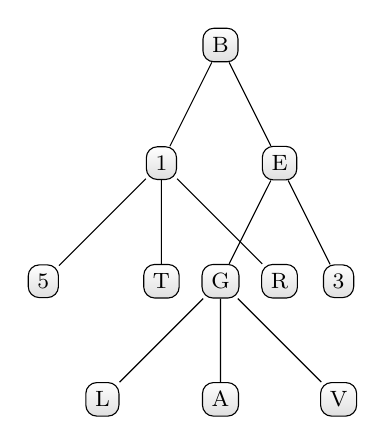
\begin{tikzpicture}[every node/.style = {shape=rectangle,rounded corners,draw, align=center, top color=white, bottom color=gray!25, font=\footnotesize}]]
		\node {B}
		child { node {1}
			child { node {5} }
			child { node {T} }
			child { node {R} }
		}
		child { node {E}
			child { node {G}
				child { node {L} }
				child { node {A} }
				child { node {V} }
			}
			child { node {3} }
		};
		\end{tikzpicture}}
\end{tabular}}
\ans{a) 3, b) 2, c) 5TR1LAVG3EB}


\exe{Gradnja min kopice z zaporednim vstavljanjem.
\begin{enumerate}
	\item Zgradi min kopico z zaporednim vstavljanjem števil iz naslednjega zaporedja
	$$ 9,3,1,9,7,6,2,7,5. $$
	Izriši drevo vsakič, ko vstaviš element v kopico. Jasno označi kopice.
	\item Koliko (natančno) zamenjav se opravi v \textbf{najslabšem} primeru in koliko v \textbf{najboljšem} primeru pri vstavljanju $i$-tega elementa? Namig: elemente začni šteti z 1.
	\item Zapiši primer zaporedij dolžine pet, kjer pride do najslabšega in do najboljšega primera.
	\item Zapiši asimptotično časovno zahtevnost v najslabšem primeru za takšen način gradnje.
	\item Zapiši algoritem, ki v konstantnem času vrne \textbf{drugi} najmanjši element kopice.
\end{enumerate}}
\ans{a) 3 b) 3 c) 2 d) 2}


\section{Namigi in rešitve izbranih nalog}

\shipoutAnswer